
\documentclass[8pt]{article}

\usepackage[utf8]{inputenc}

\usepackage{amsmath}
\usepackage{graphicx}
\usepackage{amssymb}
\usepackage{float}
% set font size to 11pt


\setlength{\parskip}{\baselineskip}%
\setlength{\parindent}{0pt}%

\begin{document}

% insert pdf cover page here

\title{Extended Coursework Report}
\author{lwp26}
\date{Feburary 2023}
\maketitle

\begin{abstract}
    \centering
    % Optimisation of tuned dampers to reduce the amplitude of resonant responses of a 3 degree of freedom structure
    In this report a model structure with 3 degrees of freedom will be hamonically excited to determine the resonant frequencies and mode shapes of the structure.
    The resonant frequnencies and mode shapes will be used to determine optimal design parameters for three seperate absorbers to reduce the resonant responses at each mode shape.
    % The optimal design parameters will be determined by using a genetic algorithm to minimise the resonant response of the structure.
    This approach can be used on real structures to reduce the amplitude of their resonant response to earthquakes.
\end{abstract}

\section{Introduction}

% Aims, Objectives and context
% context

Modern structures are designed to withstand a range of distributed static loads however they are vulnerable to harmonic excitations such as earthquakes.


\subsection{Aims}

\begin{itemize}
\item To determine the resonant frequencies of a 3 degree of freedom structure
\item To determine the properties of three seperate tuned mass dampers to reduce the three resonant response of the structure
\item To investigate the combined effect of the tuned mass dampers on the resonant response of the structure
\end{itemize}

\newpage

\section{Results}

\begin{figure}[H]
    
    \centering
    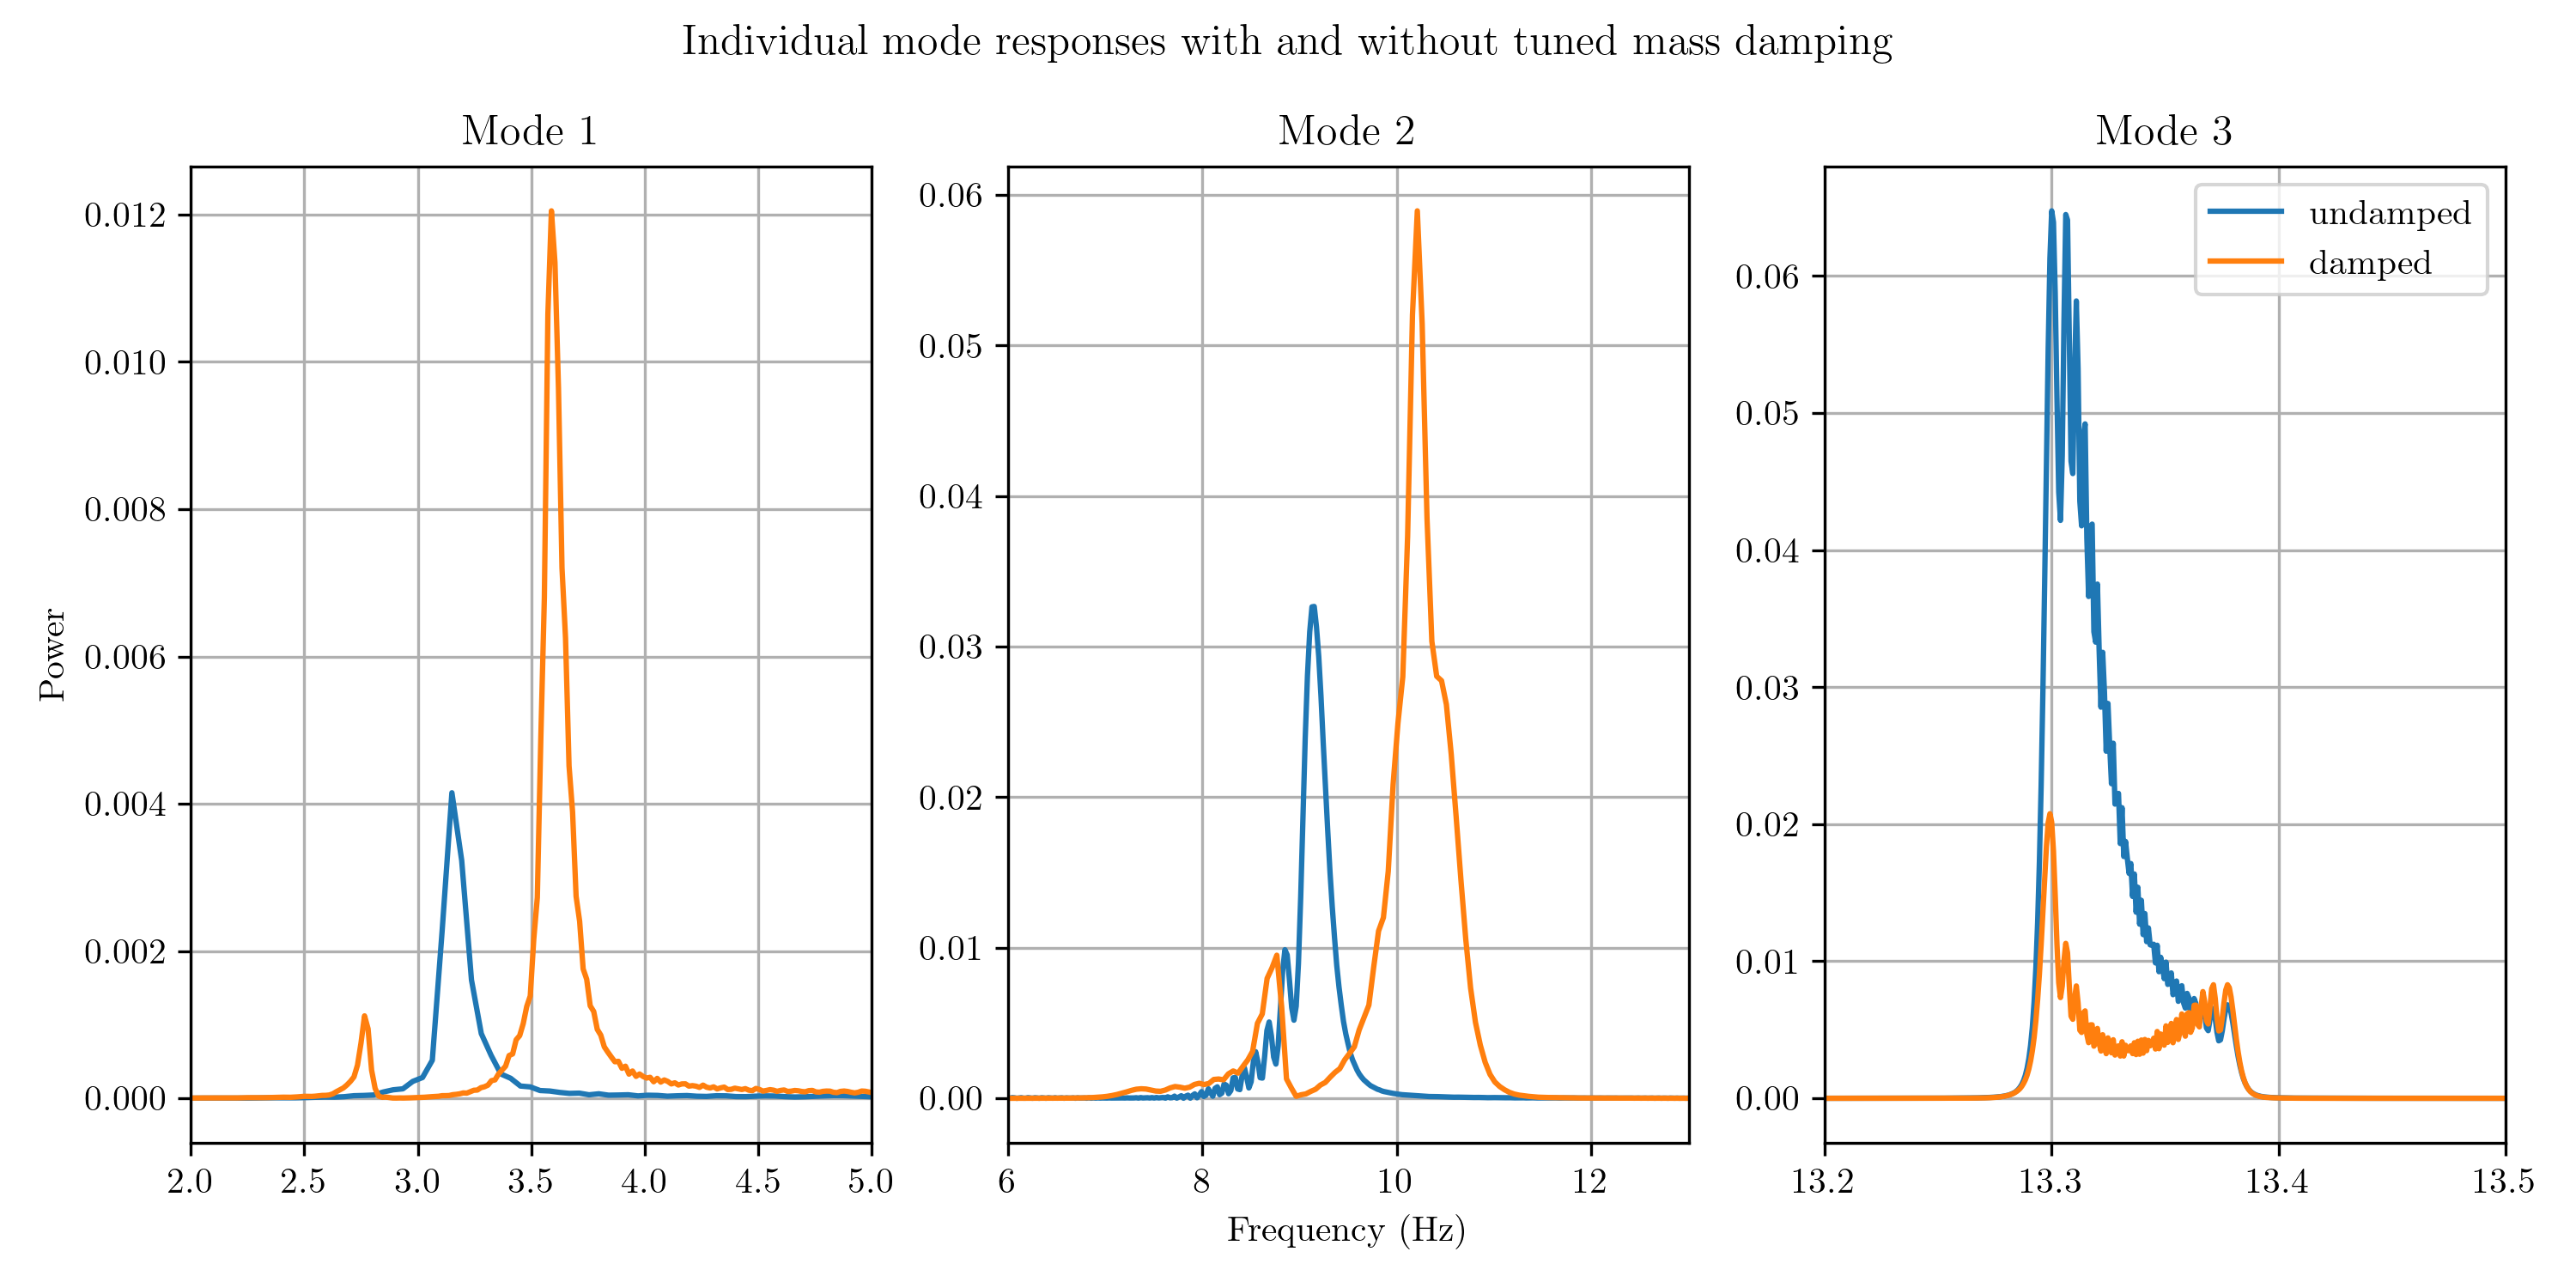
\includegraphics[width=1\textwidth]{modes.png}
    \caption{\label{fig:modes} Harmonic responses of each node before and after the addition of a single tuned damper to that node}
    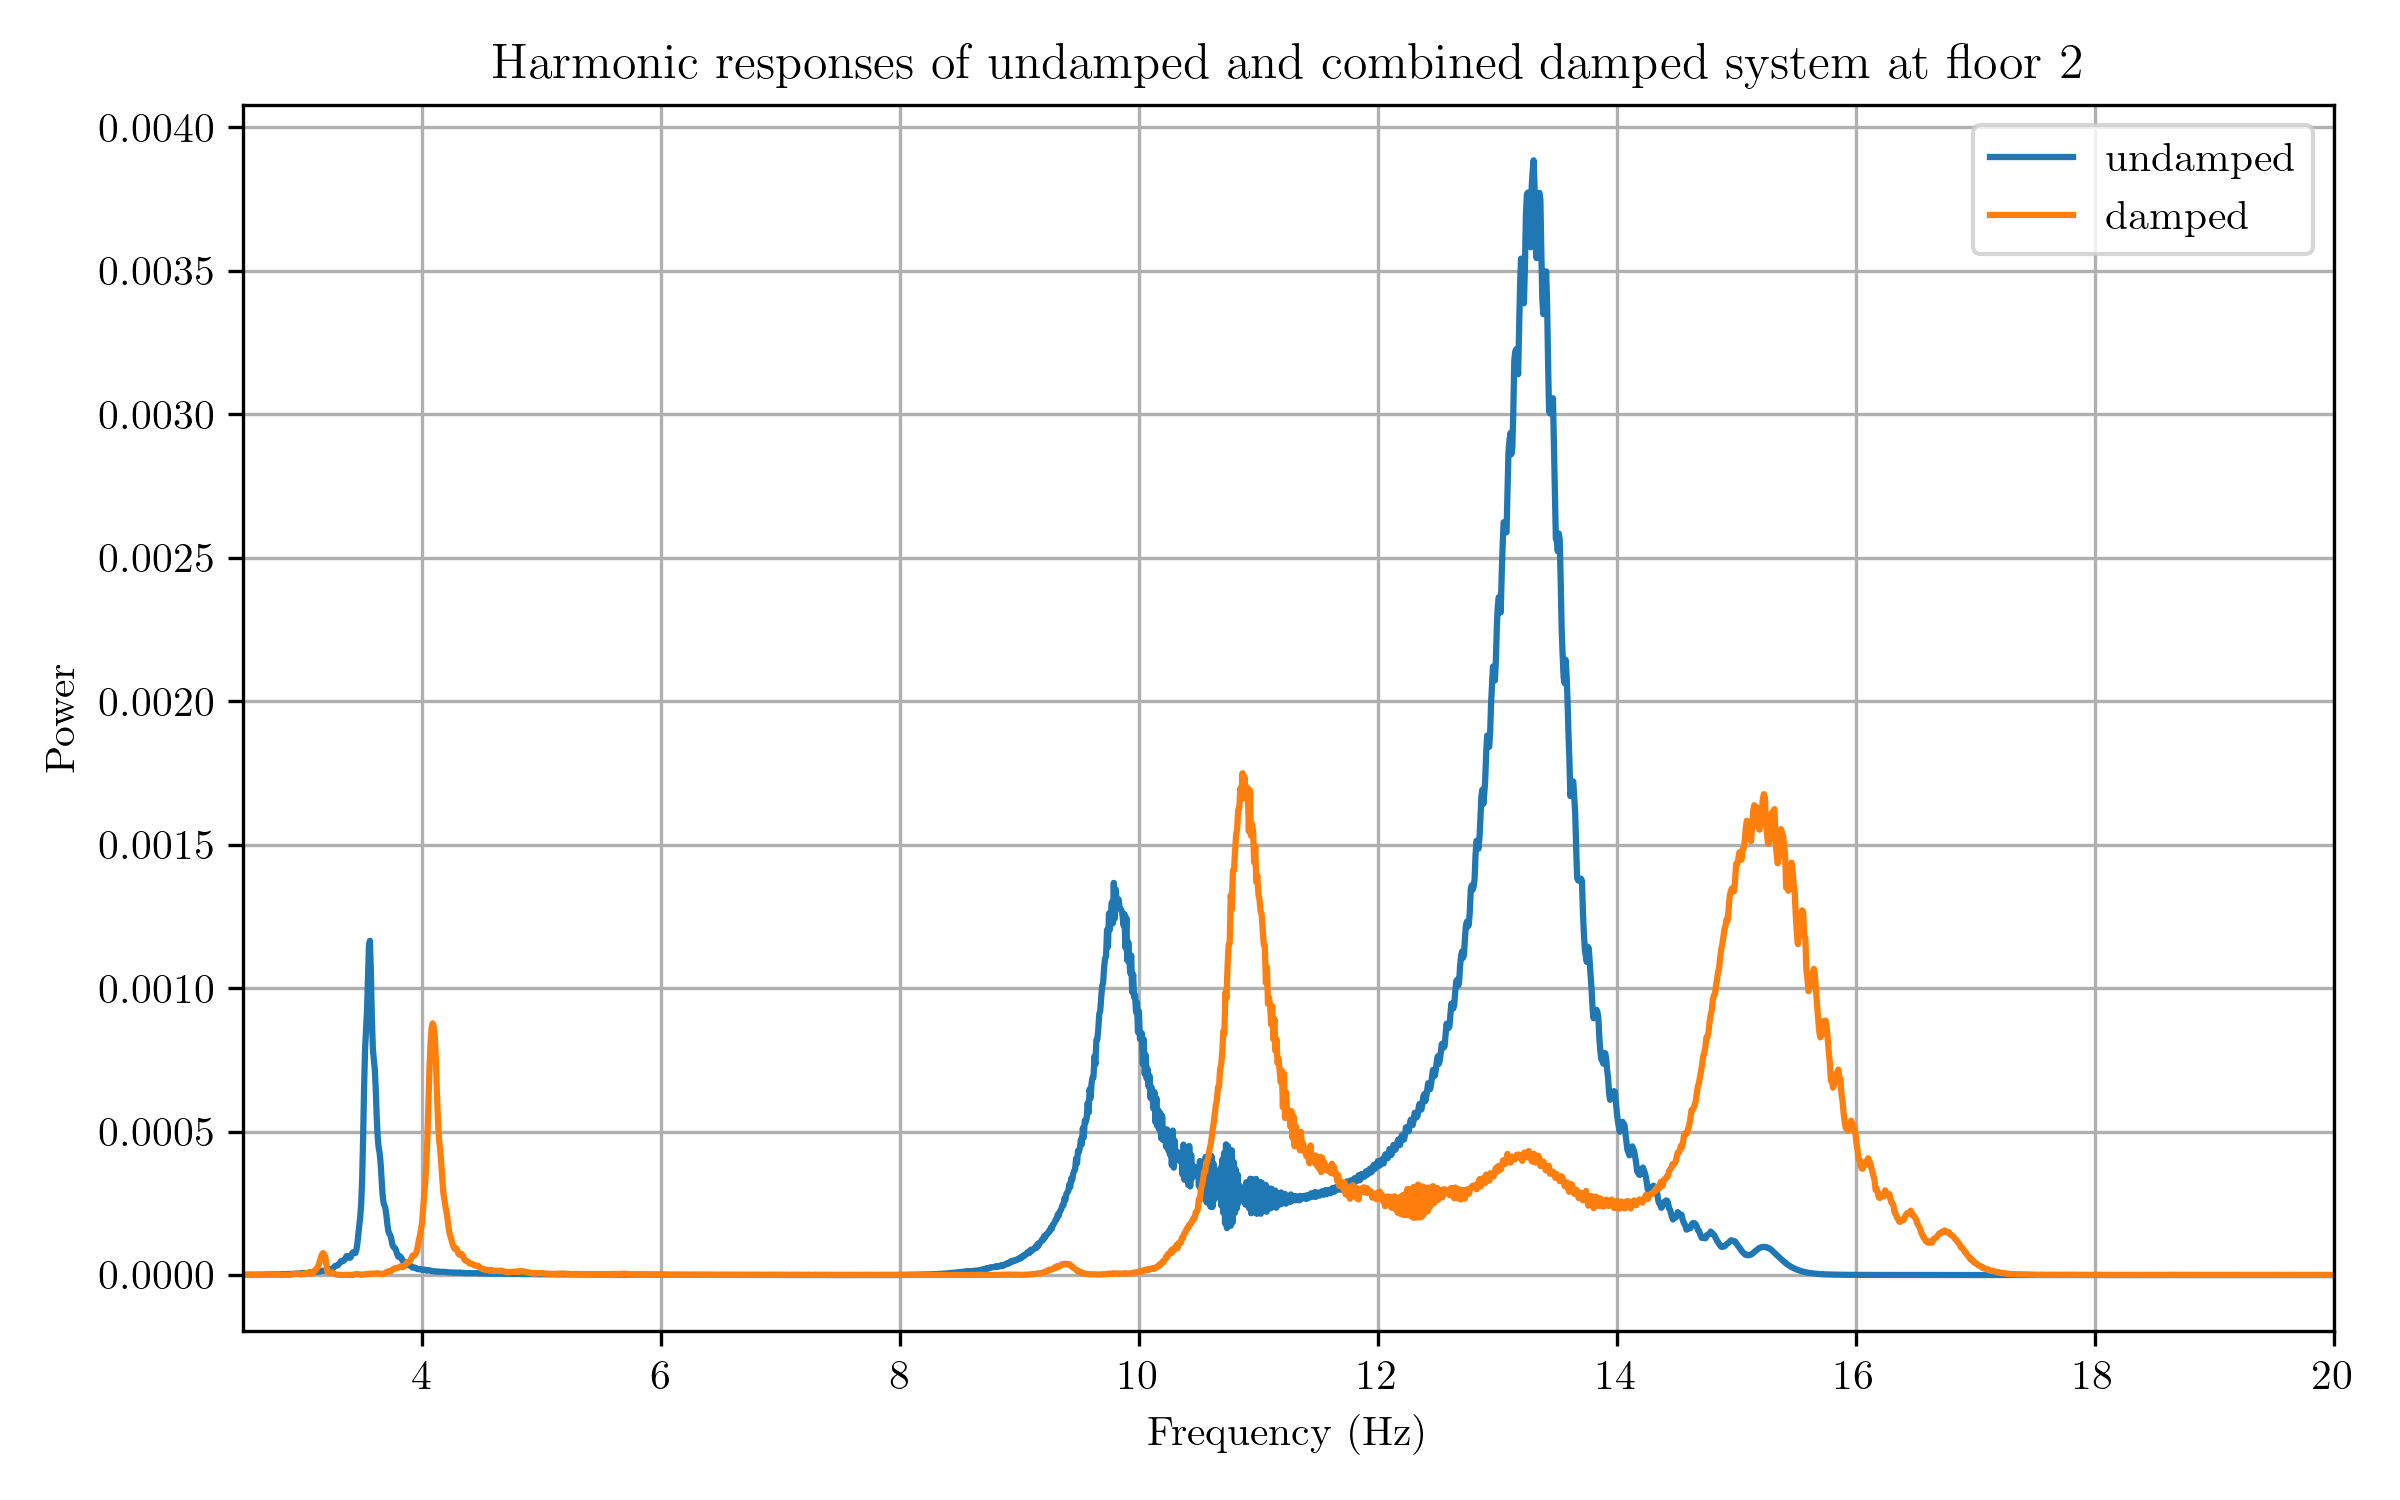
\includegraphics[width=0.8\textwidth]{combined_full_sweep.png}
    \caption{\label{fig:combined_full_sweep} Harmonic response of structure before and after the addition of 3 tuned dampers}
\end{figure}

\newpage
\section{Discussion}
%interpret results and comment on anomalies

Figure \ref{fig:modes} shows the resonant response of each mode before and after the addition of a tuned mass damper.
In all cases the response at the resonant frequency is reduced by the addition of the tuned mass damper. It can also be seen that the
response slightly above and below the resonant frequency increases. This is the expected behaviour from adding a tuned mass damper.
However, in modes 1 and 2 the new resonant response is greater than the original response.

This is likely due to a variety of reasons:
\begin{itemize}
    \item The tuned mass dampers were not accurately tuned to the resonant frequency of the structure. Our tuning method was not optimal as the length of the cantilever was only tuned to the nearest 5mm.
            This was done to reduce the time taken to tune the dampers as the tuning method was already very time consuming.
    \item The damping of the masses is very small as the air friction is negligible. This means that the two residual resonant responses are much higher than they would be if the absorbers had damping.
\end{itemize}

Figure \ref{fig:combined_full_sweep} shows the resonant response of the structure before and after the addition of the 3 individually tuned mass dampers.
Second order effects are seen in the response of the damped structure.

\section{Improvements}

The tuning method used to tune the tuned mass dampers was not optimal and could be improved.
This could be done by tuning the length of the cantilever to a higher precision using callipers.

Damping is, as mentioned in the discussion, a major factor in the resonant response of the structure and so
a major improvement would be to add damping to the tuned mass dampers. This could be done in our case 
by adding plates of varying areas to the masses to increase the damping due to air resistance.
This is still not ideal however as the damping coefficient would depend on $v^2$ of the mass and so would not produce a consistent response.
A better method would be to use a viscous damper which can be adjusted to tune an optimal damping coefficient.

\section{Conclusion}

From the experimental data gathered it can be concluded that tuned mass dampers can be used to reduce the amplitude of resonant responses of a structure.
However, tuning such dampers to the resonant frequency of the structure is not trivial and requires a lot of experimentation.

\end{document}
